% BÀI TOÁN HÌNH HỌC - BAI_HINH_17 (TRÍCH ĐỀ 17)
\begin{ex}
% Câu 13
	Cho tam giác $ABC$ nhọn, nội tiếp đường tròn $(O)$. Các đường cao $AD, BE, CF$ cắt nhau tại $H$.
	\begin{enumerate}
		\item[a)] Chứng minh 4 điểm $B, C, E, F$ cùng thuộc một đường tròn.
		\item[b)] Chứng minh: $AF \cdot AB = AE \cdot AC$.
	\end{enumerate}
\loigiai{
{
	\begin{center}
		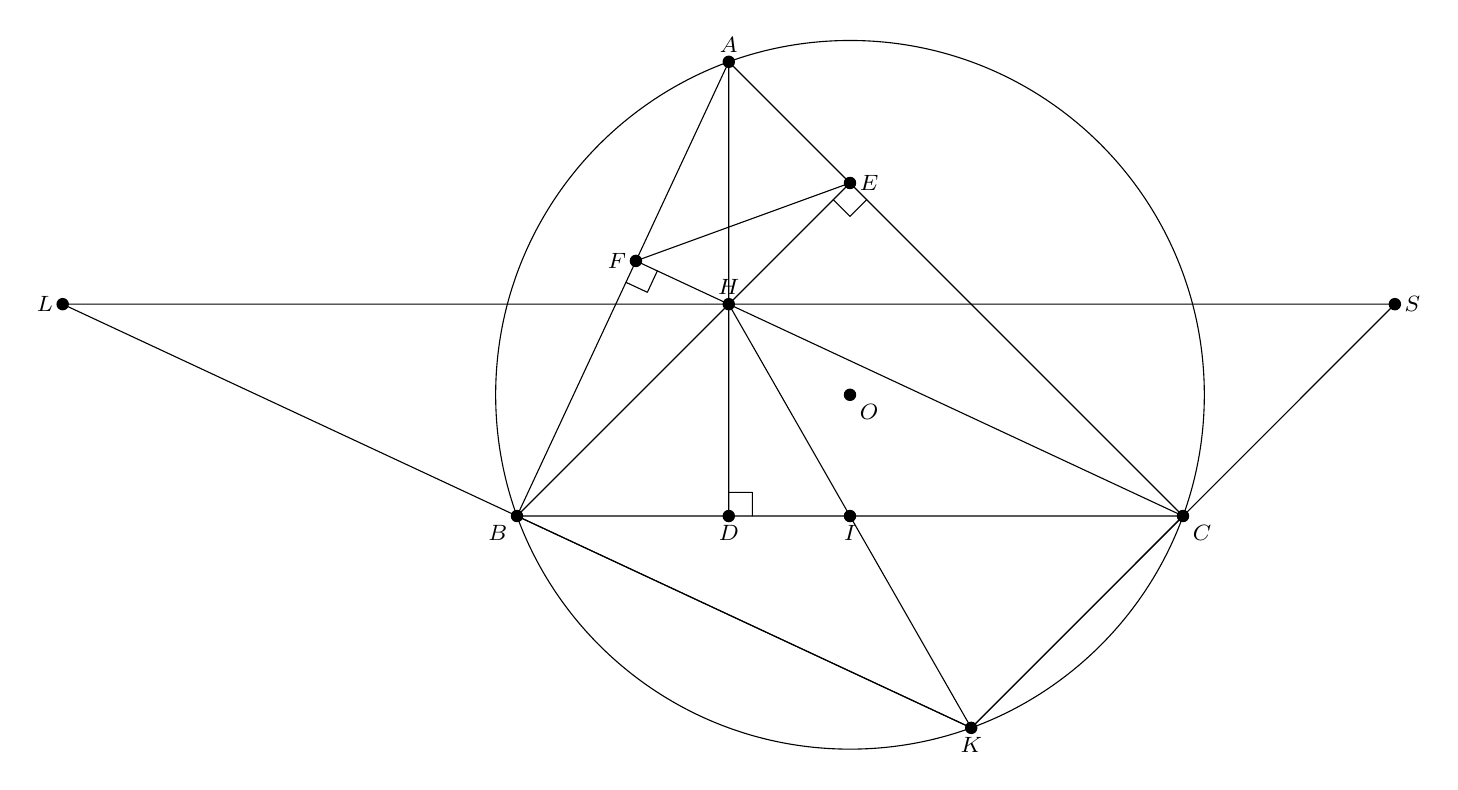
\begin{tikzpicture}[line join = round, line cap=round,>=stealth,font=\footnotesize,scale=1.5]
			\usetikzlibrary{calc,intersections,angles}
			
			% Khai báo hằng số
			\def\r{3} % r = 3cm
			
			% Định nghĩa tọa độ các điểm ban đầu
			\coordinate (O) at (0,0);
			\coordinate (B) at (-160:\r); 
			\coordinate (C) at (-20:\r);  
			\coordinate (A) at (110:\r); 
			
			% D là hình chiếu của A lên BC
			\coordinate (D) at ($(B)!(A)!(C)$);
			% E là hình chiếu của B lên AC
			\coordinate (E) at ($(A)!(B)!(C)$);
			% F là hình chiếu của C lên AB
			\coordinate (F) at ($(A)!(C)!(B)$);
			
			% H là giao điểm của BE và CF
			\path[name path=lineBE_H] (B) -- (E);
			\path[name path=lineCF_H] (C) -- (F);
			\path[name intersections={of=lineBE_H and lineCF_H, by=H}];
			
			% I là trung điểm của BC
			\coordinate (I) at ($(B)!0.5!(C)$);
			
			% Lấy điểm K sao cho O là trung điểm của AK (K = 2*O - A)
			\coordinate (K) at ($2*(O)-(A)$);
			% Lấy điểm L sao cho B là trung điểm của LK (L = 2*B - K)
			\coordinate (L) at ($2*(B)-(K)$);
			% Lấy điểm S sao cho C là trung điểm của SK (S = 2*C - K)
			\coordinate (S) at ($2*(C)-(K)$);
			
			% Vẽ các đối tượng hình học
			\draw (O) circle (\r);          % Đường tròn (O;r)
			\draw (A) -- (B) -- (K) -- (C) -- cycle; % Đa giác A-B-K-C-A (A-B-K-C là tứ giác, cycle sẽ nối C với A)
			\draw (B) -- (C) -- (F) -- (E) -- cycle; % Đa giác B-C-F-E-B
			\draw (A) -- (D);  
			\draw (L) -- (K);              % Đoạn A-D
			\draw (H) -- (K) -- (S) -- (L) -- cycle; % Đa giác H-K-S-L-K
			
			% Tô màu cho các điểm (theo cấu trúc đầu tiên)
			\fill (O) circle (1.5pt);
			\fill (A) circle (1.5pt);
			\fill (B) circle (1.5pt);
			\fill (C) circle (1.5pt);
			\fill (D) circle (1.5pt);
			\fill (E) circle (1.5pt);
			\fill (F) circle (1.5pt);
			\fill (H) circle (1.5pt);
			\fill (I) circle (1.5pt);
			\fill (K) circle (1.5pt);
			\fill (L) circle (1.5pt);
			\fill (S) circle (1.5pt);
			
			% Đặt nhãn cho các điểm (theo cấu trúc đầu tiên)
			\node[below right] at (O) {$O$};
			\node[above] at (A) {$A$};
			\node[below left] at (B) {$B$};
			\node[below right] at (C) {$C$};
			\node[below] at (D) {$D$};      
			\node[right] at (E) {$E$};      
			\node[left] at (F) {$F$};      
			\node[above] at (H) {$H$};      
			\node[below] at (I) {$I$};
			\node[below] at (K) {$K$};
			\node[left] at (L) {$L$};
			\node[right] at (S) {$S$};
			
			% Ký hiệu các góc vuông mới
			\pic[draw, angle radius=3mm]{right angle = B--F--C}; 
			\pic[draw, angle radius=3mm]{right angle = B--E--C}; 
			\pic[draw, angle radius=3mm]{right angle = A--D--C}; 
			
		\end{tikzpicture}
		
	\end{center}
}
\end{ex}
